
%----------------------------------------------------------------------------------------
%	Lecture 8
%----------------------------------------------------------------------------------------

\chapter{Lagrange Multiplies}

\bigbreak

We looked at min/max problems ealier but in that case all the variables were independent.
Here, we will try to minimize / maximize a function $f(x, y, z)$ given a contraint $g(x, y, z) = c$.

One way to do this is to solve for one variable using the contraint and then substitute. 
Then your function will become a function of two independent variables. But sometimes it is not possible to do that.
So we need a new method.

We can't use critical points of $f$ because typically they don't satisfy the constraint.


{\bf Example : } Let's say we want to find the point closest to the origin on the hyperbola $xy = 3$.

It means that we want to minimize $d(x, y) = \sqrt{x^2 + y^2}$. 
But we can also minimize the square of the distance.
So we want to minimize $f(x, y) = x^2 + y^2$ with the contraint $g(x, y) = xy = 3$.
We can start by plotting the contour plot of $f$ and $xy = 3$.

\begin{figure}[ht!]
    \centering
    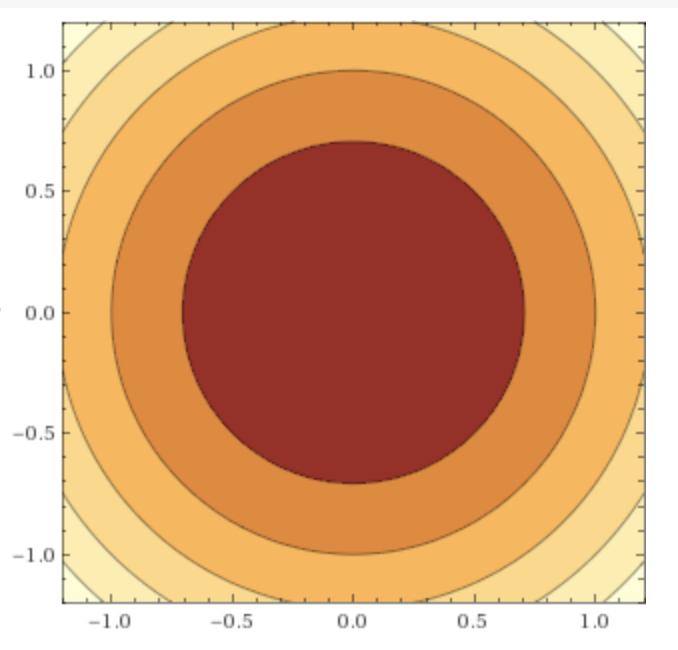
\includegraphics[scale=0.7]{./images/lecture_8_figure_1.png}
    \caption{Contour Plot of $x^2 + y^2$}
\end{figure}

We can slowly increase the value of $f$ until it touches the hyperbola $xy = 3$.
That will be our smallest value of $f$ with constraints $xy = 3$.
This happens when the circle is tangent to the hyperbola.

The key observation is that when we have a minima then the level curve of $f$ is tangent to the constraint $g$.

{\bf How do we find the point at which the the level curve is tangent to the constraint?}

Well, if they are tangent then they have the same tangent line so they will have the same normal vectors.
So, $\nabla f \parallel \nabla g$. Two vectors are parallel if they are proportionals to each other. 
So, one vector can be written as scalar multiple of the other.
$$ \nabla f = \lambda \nabla g $$

We have min/max in two variables with a contraint becomes a system of equations in three variables.

$$
    f_x  = \lambda g_x ; \quad
    f_y  = \lambda g_y ; \quad
    g  = c
$$

There is no general method to solve these equations.

Now, from our example we have $f_x = 2x, f_y = 2y, g_x = y, g_y = x$. So we have to solve
$$
    2x = \lambda y ; \quad
    2y = \lambda x ; \quad
    xy = 3 
$$
This system can be easily solved by multiplying the first two equations to get $4xy = \lambda ^ 2 xy$. 
Now substitute $xy = 3$ so $\lambda ^ 2 = 4 \implies \lambda = \pm 2$. So either $x = y$ or $x = -y$.
But $x = -y$ does not work because that gives us $-y^2 = 3$. 
And $x = y$ gives us $y^2 = 3$ so, $x = y = \pm \sqrt{3}$.


\subsection*{Why is this method valid?}

At constrained minima/maxima, the rate of change of $f$ must be zero in any direction along the level $g = c$.
We can say the same thing in terms of directional derivatives.

For any $\hat{u}$ tangent to the level $g = c$, we must have \ilds{ \diff{f}{s}\Big|_{\hat{u} = 0} }. 
Now the directional derivative is $(\nabla f) \cdot \hat{u}$. So any $\hat{u}$ must be perpendicular to $\nabla f$.

That means that $\nabla f$ is perpendicular to the level $g = c$. 
But we know another vector that is perpendicular to the level $g = c$ and that is  $\nabla g$.
So $\nabla f \parallel \nabla g$ because both are perpendicular to the level $g = c$.


{\bf Note : } The points found via this method do not guarantee minima or maxima. 
We cannot use the second derivative test to determine it. It just tells you the critical points.
You'll have to check each point whether it is a maxima, a minima or a saddle point.
